%!TEX program = xelatex
% =============================================================================
% PRESENTACIÓN — Evaluación 3 ECSD · Caso 2: Línea de Producción con Balanceo Dinámico
%
% FORMATO B (alternativa a presentacion_caso2.tex)
%
% Diferencias respecto del formato A:
%   · Sin numeración de temas. La orientación la dan cuatro láminas de acto
%     (fondo tinta) que parten la charla, no un contador que se desincroniza
%     de las páginas.
%   · Encabezado editorial: antetítulo espaciado + titular en caja mixta con
%     tipografía Light y barra de acento vertical, en vez de título en
%     versalitas precedido de un número gigante.
%   · Menos texto por lámina: una idea, su evidencia, y una franja «clave»
%     con la frase que hay que decir en voz alta.
%   · Misma paleta que las figuras del informe (color = importancia, no
%     identidad), así que los PDF vectoriales entran sin retoque.
%
% CÓMO COMPILARLO
%   · Local:    xelatex presentacion_caso2_alt.tex  (dos pasadas)
%   · Overleaf: subir el repositorio completo y elegir XeLaTeX en Menú →
%               Compiler. La primera línea de este archivo ya lo pide.
%     En Overleaf no existen las fuentes de Microsoft, así que el bloque de
%     tipografía cae solo a Lato + Roboto Condensed, que sí están ahí.
%
% Las figuras se generan con informe/figuras/generar_figuras.py
% =============================================================================
\documentclass[aspectratio=169,10pt]{beamer}

\usepackage[spanish, es-tabla]{babel}
\deactivatequoting
\usepackage{graphicx}
\usepackage{booktabs}
\usepackage{tikz}
\usetikzlibrary{shapes.geometric, arrows, positioning, calc}

\usepackage{fontspec}

% ── Tipografía, en cascada de tres niveles ───────────────────────────────────
% El diseño necesita tres cosas: una sans con peso Light para los titulares,
% una Semibold para los antetítulos espaciados, y una condensada para las
% cifras grandes. Se buscan en este orden:
%
%   1. Fuentes de Windows — Segoe UI Light/Semibold + Bahnschrift.
%      Es el diseño original; sale así compilando en la máquina de cualquiera
%      de los dos.
%   2. Fuentes libres del árbol de TeX Live — Lato (tiene Light y Semibold) y
%      Roboto Condensed. Es lo que hay en Overleaf, que no trae las de
%      Microsoft. Sin esto, allá caería todo a Latin Modern y el diseño se
%      desarma.
%   3. Las genéricas de LaTeX, para que la compilación nunca falle por fuentes.
%
% Los paquetes `lato` y `roboto` vienen en TeX Live completo (Overleaf los
% tiene); las llamadas por nombre de archivo evitan depender de fontconfig.
\newif\ifhaysegoe  \IfFontExistsTF{Segoe UI Light}{\haysegoetrue}{\haysegoefalse}
\newif\ifhaylato   \IfFontExistsTF{Lato-Light.ttf}{\haylatotrue}{\haylatofalse}

\ifhaysegoe
  \setsansfont{Segoe UI}
  \newfontfamily\ligera{Segoe UI Light}
  \newfontfamily\antetitulo{Segoe UI Semibold}[LetterSpace=16]
\else
  \ifhaylato
    \setsansfont{Lato}[
      Extension = .ttf, UprightFont = *-Regular, BoldFont = *-Bold,
      ItalicFont = *-Italic, BoldItalicFont = *-BoldItalic]
    \newfontfamily\ligera{Lato}[
      Extension = .ttf, UprightFont = *-Light, BoldFont = *-Regular,
      ItalicFont = *-LightItalic]
    \newfontfamily\antetitulo{Lato}[
      Extension = .ttf, UprightFont = *-Semibold, BoldFont = *-Bold,
      LetterSpace = 16]
  \else
    \newcommand{\ligera}{\sffamily}
    \newcommand{\antetitulo}{\sffamily\bfseries}
  \fi
\fi

% Condensada para las cifras: Bahnschrift (Windows) o Roboto Condensed (TeX Live).
\IfFontExistsTF{Bahnschrift}
  {\newfontfamily\cifrafont{Bahnschrift}}
  {\IfFontExistsTF{RobotoCondensed-Regular.ttf}
    {\newfontfamily\cifrafont{RobotoCondensed}[
       Extension = .ttf, UprightFont = *-Regular, BoldFont = *-Bold]}
    {\newcommand{\cifrafont}{\sffamily}}}

% Monoespaciada para los comandos: Fira Mono si está, si no la que haya.
\IfFontExistsTF{Consolas}
  {\setmonofont{Consolas}[Scale=0.92]}
  {\IfFontExistsTF{FiraMono-Regular.otf}
    {\setmonofont{FiraMono}[
       Extension = .otf, UprightFont = *-Regular, BoldFont = *-Bold, Scale=0.92]}
    {}}

% Las figuras se buscan igual si se compila desde presentacion/ o desde la raíz
% del repositorio, y también si en Overleaf se sube todo aplanado.
\graphicspath{{../informe/figuras/}{informe/figuras/}{figuras/}{./}}

% ── Colores: los mismos de informe/figuras/generar_figuras.py ────────────────
\definecolor{tinta}{HTML}{1C2026}      % texto principal
\definecolor{tinta2}{HTML}{52514E}     % texto secundario
\definecolor{suave}{HTML}{898781}      % pies y etiquetas menores
\definecolor{grilla}{HTML}{E1E0D9}     % filetes
\definecolor{grisclaro}{HTML}{EDECE7}  % fondo de bloque
\definecolor{tealu}{HTML}{009B8A}      % acento USACH
\definecolor{ambar}{HTML}{E8A013}      % advertencia
\definecolor{rojo}{HTML}{D03B3B}       % crítico

% ── Beamer: quitar todo lo que no informe ────────────────────────────────────
\setbeamertemplate{navigation symbols}{}
\setbeamertemplate{frametitle}{}
\setbeamercolor{normal text}{fg=tinta}
\setbeamercolor{itemize/enumerate body}{fg=tinta}
\setbeamercolor{itemize/enumerate subbody}{fg=tinta2}
\setbeamerfont{normal text}{size=\small}
\setbeamertemplate{itemize item}{\textcolor{tealu}{\raisebox{0.15ex}{\tiny$\blacksquare$}}}
\setbeamertemplate{itemize subitem}{\textcolor{suave}{--}}
\setbeamercolor{bloque}{bg=grisclaro}

% El pie dice en qué acto estamos, no cuánto falta. Se fija en cada divisoria.
\newcommand{\actoactual}{}
\setbeamertemplate{footline}{%
  \hspace{1.25em}\raisebox{1.05em}{\tiny\color{suave}\actoactual}%
  \hfill
  \raisebox{1.05em}{\tiny\color{suave}ECSD · Evaluación 3 — Caso 2 · C. Olivares · S. García-Huidobro\hspace{1.6em}}%
  \raisebox{1.05em}{\tiny\color{suave}\insertframenumber\hspace{1.25em}}}

% ── Encabezado de lámina: antetítulo · titular · bajada, con barra de acento ─
\newcommand{\lamina}[3]{%
  \vspace{0.05cm}%
  \noindent\textcolor{tealu}{\rule[-0.92cm]{2.6pt}{1.32cm}}\hspace{0.32cm}%
  \begin{minipage}[t]{0.92\linewidth}
    {\antetitulo\scriptsize\color{tealu}\MakeUppercase{#1}}\\[4pt]
    {\ligera\fontsize{19}{22}\selectfont\color{tinta}#2}\\[4pt]
    {\footnotesize\color{tinta2}#3}
  \end{minipage}\\[0.5cm]}

% ── Lámina de acto (fondo tinta) ─────────────────────────────────────────────
\newcommand{\acto}[4]{%
  {\setbeamercolor{background canvas}{bg=tinta}
   \begin{frame}[plain]
   \vfill
   \hspace{1.5cm}\begin{minipage}{0.82\linewidth}
     {\antetitulo\scriptsize\color{tealu}\MakeUppercase{#1}}\\[12pt]
     {\ligera\fontsize{30}{34}\selectfont\color{white}#2}\\[14pt]
     {\color{tealu}\rule{2.6cm}{1.8pt}}\\[12pt]
     {\small\color{grilla}#3}\\[16pt]
     {\antetitulo\tiny\color{suave}\MakeUppercase{Expone: #4}}
   \end{minipage}
   \vfill
   \end{frame}}}

% ── Franja «clave»: la frase que hay que decir en voz alta ───────────────────
\newcommand{\clave}[1]{%
  \vspace{0.15cm}%
  \noindent\raisebox{-0.22cm}{\textcolor{tealu}{\rule{2.6pt}{0.66cm}}}\hspace{0.3cm}%
  \begin{minipage}[c]{0.93\linewidth}{\footnotesize\color{tinta}#1}\end{minipage}}

% ── Bloque lateral y cifra ───────────────────────────────────────────────────
\newcommand{\bloque}[2]{%
  \begin{beamercolorbox}[wd=\linewidth, sep=7pt]{bloque}%
  {\small\bfseries\color{tinta}#1}\\[3pt]{\footnotesize\color{tinta2}#2}%
  \end{beamercolorbox}}

\newcommand{\cifra}[2]{%
  \begin{center}{\cifrafont\fontsize{30}{32}\selectfont\color{tealu}#1}\\[3pt]
  {\scriptsize\color{tinta2}#2}\end{center}}

\tikzset{
  etapac/.style={rectangle, rounded corners=1pt, minimum width=2.05cm, minimum height=1.0cm,
                 text centered, draw=grilla, fill=grisclaro, font=\scriptsize, align=center},
  etaparc/.style={rectangle, rounded corners=1pt, minimum width=2.05cm, minimum height=1.0cm,
                  text centered, draw=tealu, fill=tealu!12, font=\scriptsize\bfseries, align=center},
  colaq/.style={rectangle, minimum width=0.95cm, minimum height=0.6cm, text centered,
                draw=grilla, fill=ambar!12, font=\tiny},
  nodo/.style={rectangle, rounded corners=1pt, draw=grilla, fill=grisclaro,
               font=\scriptsize\bfseries, inner sep=7pt},
  arrow/.style={semithick,->,>=stealth,color=tinta2},
  rep/.style={rectangle, rounded corners=1pt, draw=grilla, fill=grisclaro, font=\scriptsize,
              minimum width=1.65cm, minimum height=0.55cm},
  colabox/.style={rectangle, draw=grilla, fill=ambar!12, font=\scriptsize\bfseries,
                  minimum width=1.9cm, minimum height=0.55cm}
}

\begin{document}

% ═══ PORTADA ═════════════════════════════════════════════════════════════════
{\setbeamercolor{background canvas}{bg=tinta}
\begin{frame}[plain]
\vfill
\hspace{1.5cm}\begin{minipage}{0.85\linewidth}
{\antetitulo\scriptsize\color{tealu}\MakeUppercase{Estructura de Computadores y Sistemas Distribuidos · Evaluación 3 · Caso 2}}\\[18pt]
{\ligera\fontsize{32}{38}\selectfont\color{white}Línea de producción con\\balanceo dinámico de carga}\\[16pt]
{\color{tealu}\rule{2.6cm}{1.8pt}}\\[14pt]
{\small\color{grilla}Un sistema distribuido que simula una planta conservera, detecta su cuello\\de botella en vivo y demuestra qué pasa cuando se escala la etapa lenta}\\[22pt]
{\small\color{white}\textbf{César Olivares · Simón García-Huidobro}}\\[5pt]
{\footnotesize\color{suave}Profesor: Daniel Calderón R. · 24 de agosto de 2026}
\end{minipage}
\vfill
\end{frame}}

% ═══ ACTO I ══════════════════════════════════════════════════════════════════
\renewcommand{\actoactual}{I · El problema}
\acto{Primer acto}{El problema}
     {Qué simula el sistema, y la pregunta que la simulación tiene que responder.}
     {Simón}

% ── La línea ─────────────────────────────────────────────────────────────────
\begin{frame}
\lamina{El caso}{Cuatro etapas en serie, una replicada}
       {Planta conservera ficticia de jurel en lata de 425 g. La unidad de trabajo es el lote.}
\begin{center}
\begin{tikzpicture}[node distance=0.28cm]
  \node (q1) [colaq] {cola};
  \node (e1) [etapac, right=of q1] {\textbf{Fileteado}\\ 4 s};
  \node (q2) [colaq, right=of e1] {cola};
  \node (e2) [etaparc, right=of q2] {Envasado\\ 12 s\\ $\times$1--3 réplicas};
  \node (q3) [colaq, right=of e2] {cola};
  \node (e3) [etapac, right=of q3] {\textbf{Sellado}\\ 3 s};
  \node (q4) [colaq, right=of e3] {cola};
  \node (e4) [etapac, right=of q4] {\textbf{Esterilización}\\ 7 s};
  \draw [arrow] (q1) -- (e1); \draw [arrow] (e1) -- (q2);
  \draw [arrow] (q2) -- (e2); \draw [arrow] (e2) -- (q3);
  \draw [arrow] (q3) -- (e3); \draw [arrow] (e3) -- (q4);
  \draw [arrow] (q4) -- (e4);
\end{tikzpicture}
\end{center}
\vspace{0.2cm}
\begin{columns}[T]
\column{0.53\textwidth}
\begin{itemize}
  \item Entre etapa y etapa hay una \textbf{cola}: la fila de lotes esperando.
  \item Si a una etapa le llega trabajo más rápido de lo que procesa, su fila crece. Eso es un \textbf{cuello de botella}.
\end{itemize}
\column{0.43\textwidth}
\bloque{La pregunta del caso}{¿Qué le pasa al cuello de botella cuando escalas la etapa lenta?}
\end{columns}
\clave{\textbf{Adelanto:} el cuello no desaparece — \textbf{se muda}. Todo lo que sigue es la evidencia de esa frase.}
\end{frame}

% ═══ ACTO II ═════════════════════════════════════════════════════════════════
\renewcommand{\actoactual}{II · Cómo está construido}
\acto{Segundo acto}{Cómo está construido}
     {Cinco servicios, tres nodos, y una decisión de diseño que sostiene todo el resto.}
     {César}

% ── Arquitectura ─────────────────────────────────────────────────────────────
\begin{frame}[fragile]
\lamina{Arquitectura}{Tres nodos, y un mismo programa desplegado cuatro veces}
       {Cada nodo agrupa lo que escala por el mismo motivo. Las cuatro estaciones son una sola imagen.}
\begin{center}
\begin{tikzpicture}[node distance=0.4cm and 0.85cm]
  \node (na) [nodo, minimum width=3.2cm, minimum height=1.9cm,
              label={[font=\scriptsize\bfseries\color{tealu}]above:NODO A — operación}] {};
  \node at (na.center) [align=center, font=\scriptsize] {Tablero (Streamlit)\\ orders-api (FastAPI)};
  \node (nb) [nodo, right=of na, minimum width=3.7cm, minimum height=1.9cm,
              label={[font=\scriptsize\bfseries\color{tealu}]above:NODO B — procesamiento}] {};
  \node at (nb.center) [align=center, font=\scriptsize] {fileteado · sellado\\ esterilización\\ envasado $\times$1--3};
  \node (nc) [nodo, right=of nb, minimum width=3.2cm, minimum height=1.9cm,
              label={[font=\scriptsize\bfseries\color{tealu}]above:NODO C — estado}] {};
  \node at (nc.center) [align=center, font=\scriptsize] {Redis (colas)\\ metrics-api\\ SQLite};
  \draw [arrow, <->] (na) -- (nb);
  \draw [arrow, <->] (nb) -- (nc);
  \draw [arrow, <->] (na.south) to[bend right=14] (nc.south);
\end{tikzpicture}
\end{center}
\vspace{0.15cm}
\begin{columns}[T]
\column{0.56\textwidth}
\begin{itemize}
  \item \textbf{B} es lo único que se replica bajo carga; \textbf{C} concentra el estado compartido, que no puede duplicarse sin coordinación; \textbf{A} escala con los usuarios.
  \item Las cuatro estaciones son \textbf{el mismo código}: etapa, colas y tiempo de ciclo llegan por variables de entorno.
\end{itemize}
\column{0.40\textwidth}
\begin{beamercolorbox}[wd=\linewidth, sep=7pt]{bloque}
{\footnotesize\ttfamily\color{tinta}docker compose up -d\\ \hspace*{1em}--scale envasado=3}
\end{beamercolorbox}
\vspace{0.1cm}
\cifra{1 imagen}{4 etapas · hasta 6 contenedores de estación}
\end{columns}
\clave{Separar nodos separa dominios de falla: si las estaciones saturan la CPU, el operador sigue atendido.}
\end{frame}

% ── Balanceo por demanda ─────────────────────────────────────────────────────
\begin{frame}
\lamina{Balanceo}{Las réplicas piden trabajo; nadie se lo asigna}
       {El enunciado pide «réplicas detrás de un balanceador». Nuestro balanceador es la cola compartida.}
\begin{columns}[T]
\column{0.54\textwidth}
\begin{itemize}
  \item Un round-robin es \emph{estático}: le sigue mandando lotes a la réplica lenta o atascada.
  \item Con reparto por demanda, la réplica lenta \textbf{pide menos veces}.
\end{itemize}
\vspace{0.15cm}
\bloque{La cola es el punto único}{Por ella pasa todo el trabajo y ella decide quién procesa qué. Es lo que hace un balanceador, sin un proceso que lo haga.}
\column{0.42\textwidth}
\begin{center}
\begin{tikzpicture}
  \node (cola) [colabox, minimum width=2.6cm] at (0,1.45) {cola: \#7 \#8 \#9};
  \node (r1) [rep] at (-1.85,0) {réplica 1};
  \node (r2) [rep] at (0,0) {réplica 2};
  \node (r3) [rep] at (1.85,0) {réplica 3};
  \draw [arrow, <-] (cola.south west) -- (r1.north) node[font=\tiny, midway, left=1pt] {pido};
  \draw [arrow, <-] (cola.south) -- (r2.north) node[font=\tiny, midway, right=1pt] {pido};
  \draw [arrow, <-] (cola.south east) -- (r3.north) node[font=\tiny, midway, right=1pt] {pido};
  \node [font=\tiny\color{tinta2}, align=center] at (0,-0.72) {cada una reclama un lote\\ solo cuando queda libre};
\end{tikzpicture}
\end{center}
\end{columns}
\end{frame}

% ── Condición de carrera ─────────────────────────────────────────────────────
\begin{frame}
\lamina{Condición de carrera}{La provocamos antes de resolverla}
       {Las dos versiones están en el historial de commits: primero la rota, después la correcta.}
\begin{center}
\begin{tikzpicture}
  \node [font=\scriptsize\bfseries\color{rojo}] at (0,1.95) {Ingenua: mirar y sacar (2 pasos)};
  \node (colaA) [colabox] at (0,1.2) {cola: lote \#42};
  \node (r1a) [rep] at (-1.5,-0.15) {réplica 1};
  \node (r2a) [rep] at (1.5,-0.15) {réplica 2};
  \draw [arrow] (colaA.south west) -- (r1a.north) node[font=\tiny, midway, above, sloped] {ve \#42};
  \draw [arrow] (colaA.south east) -- (r2a.north) node[font=\tiny, midway, above, sloped] {ve \#42};
  \node [font=\scriptsize\bfseries\color{rojo}] at (0,-1.0) {el mismo lote, dos veces};
  \node [font=\scriptsize\bfseries\color{tealu}] at (7.6,1.95) {Atómica: \texttt{BRPOP} (1 operación)};
  \node (colaB) [colabox] at (7.6,1.2) {cola: \#42, \#43};
  \node (r1b) [rep] at (6.1,-0.15) {réplica 1};
  \node (r2b) [rep] at (9.1,-0.15) {réplica 2};
  \draw [arrow] (colaB.south west) -- (r1b.north) node[font=\tiny, midway, above, sloped] {recibe \#42};
  \draw [arrow] (colaB.south east) -- (r2b.north) node[font=\tiny, midway, above, sloped] {recibe \#43};
  \node [font=\scriptsize\bfseries\color{tealu}] at (7.6,-1.0) {0 duplicados en 200 órdenes};
\end{tikzpicture}
\end{center}
\vspace{0.1cm}
\begin{itemize}
  \item Entre «mirar» (\texttt{LRANGE}) y «sacar» (\texttt{LREM}) hay una ventana en la que otra réplica ve la misma orden. La ensanchamos a propósito hasta reproducir duplicados.
\end{itemize}
\clave{Un lock con TTL \textbf{administra} esa ventana. La extracción atómica la \textbf{elimina}: es un mutex implícito por elemento, servido por el único hilo de comandos de Redis.}
\end{frame}

% ── Criterio de cuello ───────────────────────────────────────────────────────
\begin{frame}
\lamina{El criterio}{Medimos espera, no servicio}
       {Esta decisión es el corazón del proyecto: es lo que permite ver el cuello moverse.}
\begin{columns}[T]
\column{0.46\textwidth}
\begin{itemize}
  \item En el supermercado, un cajero lento no es un atasco. El atasco es \textbf{la fila que crece} frente a su caja.
  \item Cuello = etapa con mayor \textbf{espera promedio} en una ventana móvil de 60 s, contra umbrales relativos a su propio ciclo: advertencia $\geq 1{,}5\times$, crítico $\geq 3\times$.
\end{itemize}
\column{0.50\textwidth}
\begin{center}
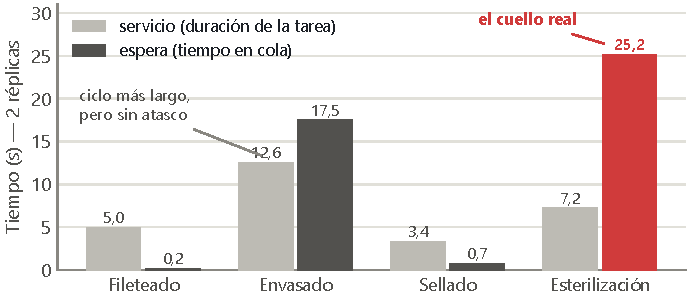
\includegraphics[width=\linewidth]{fig_espera_vs_servicio.pdf}
\end{center}
\end{columns}
\clave{Con 2 réplicas, envasado sigue teniendo el ciclo más largo (12 s) y \textbf{no} es el cuello. Midiendo servicio, el detector lo habría señalado para siempre.}
\end{frame}

% ═══ DEMO ════════════════════════════════════════════════════════════════════
\renewcommand{\actoactual}{Demo en vivo}
\acto{Interludio}{Demo en vivo}
     {El sistema completo corriendo: tablero en localhost:8501, con lotes reales entrando a la línea.}
     {Ambos}

% ── Guion de demo ────────────────────────────────────────────────────────────
\begin{frame}
\lamina{Demo}{Qué vamos a mostrar, en orden}
       {Levantado antes de empezar con \texttt{--scale envasado=2}. Aproximadamente cuatro minutos.}
\begin{columns}[T]
\column{0.56\textwidth}
{\footnotesize
\begin{enumerate}
  \item La línea al día: 4 etapas y 5 réplicas visibles, cada una con su ciclo y su carga.
  \item Ingresamos lotes desde la interfaz, espaciados unos 5 s.
  \item La espera de esterilización crece: el cartel pasa a \textcolor{ambar}{\textbf{ámbar}} y luego a \textcolor{rojo}{\textbf{rojo}}, diciendo por qué.
  \item \textbf{La carrera, en vivo}: el botón «Ejecutar la comparación» corre las dos versiones del reclamo lado a lado — 300 envasados de 100 pedidos contra 100 de 100.
  \item Matamos Redis: la interfaz \textbf{nombra al servicio caído} y el resto sigue vivo.
\end{enumerate}}
\column{0.40\textwidth}
\bloque{Es el mismo código}{La comparación importa \texttt{servicios/comun/reclamo.py}, el módulo que usan las estaciones reales. No hay una copia para la demo que pueda quedar desincronizada.}
\vspace{0.15cm}
\cifra{1 comando}{\texttt{docker compose up} — despliegue completo, sin pasos manuales}
\end{columns}
\end{frame}

% ═══ ACTO III ════════════════════════════════════════════════════════════════
\renewcommand{\actoactual}{III · Lo que medimos}
\acto{Tercer acto}{Lo que medimos}
     {Cinco experimentos reproducibles. Ninguna afirmación de aquí en adelante es una opinión.}
     {Simón}

% ── Aritmética ───────────────────────────────────────────────────────────────
\begin{frame}
\lamina{El escenario}{La aritmética antes del experimento}
       {Inyección de una orden cada 5 s durante 180 s: 12 lotes por minuto entrando a la línea.}
\begin{center}
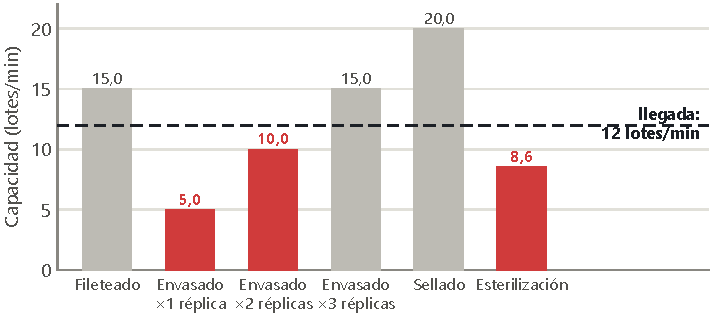
\includegraphics[width=0.64\linewidth]{fig_capacidad.pdf}
\end{center}
\clave{Toda etapa \textbf{bajo la línea de llegada} acumula fila tarde o temprano. Con 2 réplicas envasado sube a 10 lotes/min y esterilización (8,6) queda como el siguiente límite: la figura \textbf{anticipa} el resultado.}
\end{frame}

% ── Resultado central ────────────────────────────────────────────────────────
\begin{frame}
\lamina{Resultado central}{El cuello no se elimina: se muda}
       {Espera promedio por etapa, según cuántas réplicas tenga envasado.}
\begin{center}
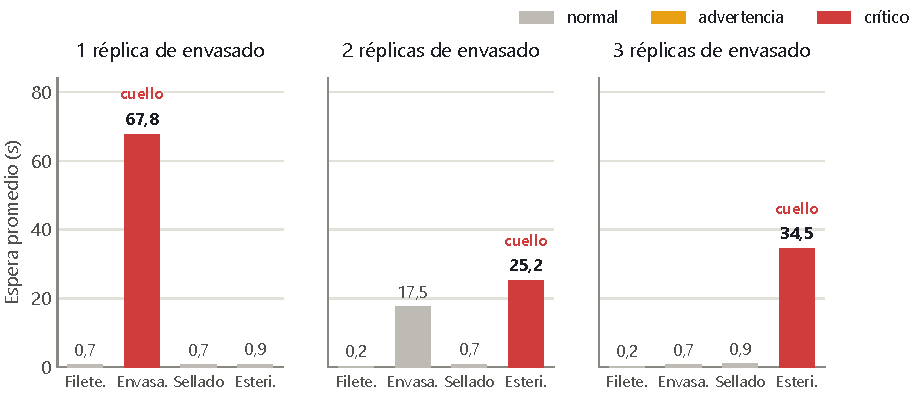
\includegraphics[width=0.78\linewidth]{fig_espera_replicas.pdf}
\end{center}
\begin{itemize}
  \item Con 1 réplica, envasado acumula \textbf{67,8 s} de espera y el resto de la línea queda casi ociosa.
  \item Con 2, el cuello \textbf{se desplaza a esterilización}. Con 3, envasado baja a 0,7 s\dots{} y el cuello sigue en esterilización.
\end{itemize}
\end{frame}

% ── Lead time ────────────────────────────────────────────────────────────────
\begin{frame}
\lamina{Rendimiento}{Cuánto compra realmente cada réplica}
       {Lead time: lo que tarda un lote desde que se crea hasta que sale terminado.}
\begin{columns}[T]
\column{0.52\textwidth}
\vspace{0.3cm}
\begin{center}
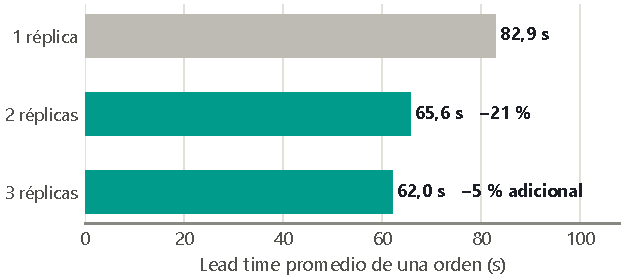
\includegraphics[width=\linewidth]{fig_leadtime.pdf}
\end{center}
\column{0.44\textwidth}
\vspace{0.2cm}
\begin{itemize}
  \item La segunda réplica compra un \textbf{21 \%} de mejora.
  \item La tercera, casi nada: el límite ya no está en envasado.
\end{itemize}
\end{columns}
\clave{La siguiente inversión correcta sería \textbf{una segunda autoclave}, no una tercera envasadora. El tablero responde eso en vivo, que es para lo que sirve.}
\end{frame}

% ── Réplica lenta ────────────────────────────────────────────────────────────
\begin{frame}
\lamina{Balanceo dinámico}{Qué pasa cuando una réplica es más lenta}
       {Dos réplicas normales más una al doble de ciclo, sobre la misma cola, 30 lotes.}
\begin{columns}[T]
\column{0.50\textwidth}
\begin{center}
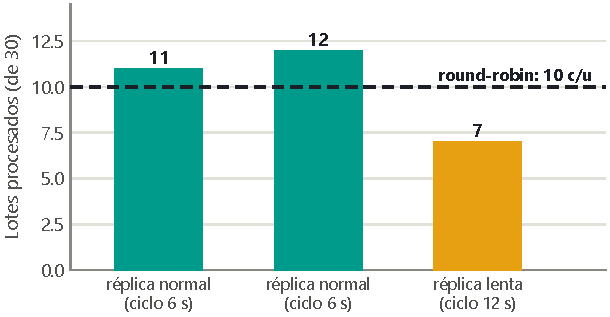
\includegraphics[width=\linewidth]{fig_replica_lenta.pdf}
\end{center}
\column{0.46\textwidth}
\vspace{0.35cm}
\begin{itemize}
  \item Un round-robin habría repartido \textbf{10 / 10 / 10} sin mirar la velocidad de nadie.
  \item El reparto medido fue \textbf{11 / 12 / 7}.
\end{itemize}
\end{columns}
\clave{Nadie programó ese reparto: salió de que cada réplica pide trabajo solo al quedar libre. Eso es balanceo \emph{dinámico} — proporcional a la capacidad real.}
\end{frame}

% ── Saturación ───────────────────────────────────────────────────────────────
\begin{frame}
\lamina{Saturación}{Se declara crítico solo, y se recupera solo}
       {Ráfaga de 25 órdenes de golpe, sondeando \texttt{/metricas/cuello} cada 15 s.}
\begin{center}
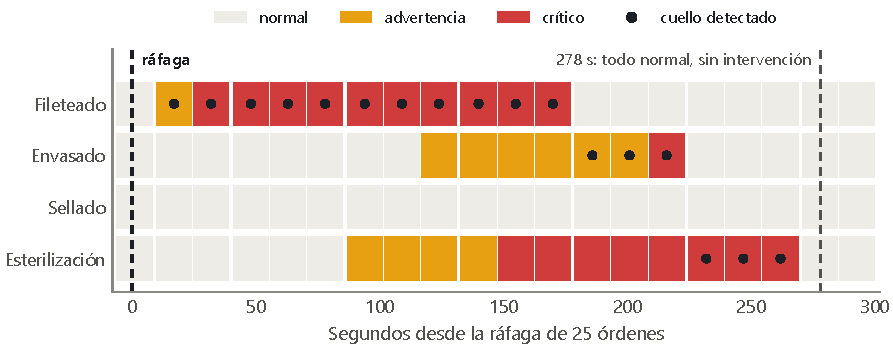
\includegraphics[width=0.76\linewidth]{fig_saturacion.pdf}
\end{center}
\clave{A los \textbf{32 s} el sistema se declara crítico sin que nadie se lo diga; la congestión recorre la línea como una ola. A los \textbf{278 s} todo vuelve a normal \textbf{sin intervención}: las esperas viejas salieron de la ventana móvil.}
\end{frame}

% ── Errores, persistencia, despliegue ────────────────────────────────────────
\begin{frame}[fragile]
\lamina{Robustez}{Errores, persistencia y despliegue}
       {Lo que el enunciado exige como base, verificado contra el sistema corriendo.}
\begin{columns}[T]
\column{0.31\textwidth}
\cifra{2,1 s}{respuesta \texttt{503} con plazo duro, nombrando al servicio caído}
{\scriptsize\color{tinta2}El hallazgo: el cuelgue de 46 s con Redis caído estaba en la resolución DNS, no en el socket.}
\column{0.31\textwidth}
\cifra{2 tablas}{\texttt{ordenes} y \texttt{eventos} — 12 eventos por orden completa}
{\scriptsize\color{tinta2}Espera, servicio y lead time \textbf{no se guardan}: se calculan desde los eventos. El dato guardado dos veces es el que se contradice.}
\column{0.31\textwidth}
\cifra{8/8}{contenedores \emph{healthy} en la prueba de clon limpio}
{\scriptsize\color{tinta2}\texttt{201} creación · \texttt{422} validación · \texttt{404} inexistente · \texttt{503} dependencia caída.}
\end{columns}
\clave{El healthcheck mide \emph{vida}, no dependencias: un servicio que responde 503 explicándose está sano. La base sobrevive a \texttt{docker compose down}.}
\end{frame}

% ═══ ACTO IV ═════════════════════════════════════════════════════════════════
\renewcommand{\actoactual}{IV · Lo que aprendimos}
\acto{Cuarto acto}{Lo que aprendimos}
     {Los límites que conocemos, y las cinco frases que resumen el proyecto.}
     {César}

% ── Resiliencia ──────────────────────────────────────────────────────────────
\begin{frame}[fragile]
\lamina{Resiliencia}{No la exige el enunciado; sabemos dónde iría}
       {La división en nodos deja los puntos de corte listos: cada mejora toca uno solo.}
\begin{itemize}
  \item \textbf{Estaciones} — sin estado propio: reconectan y mueren sin corromper nada. Pendiente: re-encolar el lote en curso si una réplica muere a mitad de ciclo (\texttt{BLMOVE} a una cola «en proceso» más un barrendero de latidos vencidos).
  \item \textbf{Redis} — punto único de falla del reparto: Redis Sentinel, o un broker con confirmaciones (ahí apuntaba el bonus de Kafka).
  \item \textbf{SQLite} — con más escritores o failover, migrar a MySQL cambiando solo \texttt{bd.py}.
  \item \textbf{APIs y tablero} — sin estado: dos instancias tras un balanceador HTTP quedan en alta disponibilidad, y los healthchecks que ya existen son su insumo.
\end{itemize}
\clave{Ninguna de estas cuatro mejoras obliga a rediseñar las otras tres. Para eso era la división en nodos.}
\end{frame}

% ── Conclusiones ─────────────────────────────────────────────────────────────
\begin{frame}
\lamina{Conclusiones}{Cinco frases, todas medidas}
       {Cada una tiene su experimento reproducible en el informe y su script en el repositorio.}
\begin{columns}[T]
\column{0.48\textwidth}
\bloque{El cuello no se elimina: se muda}{De envasado a esterilización al pasar de 1 a 2 réplicas. La tercera ya casi no compra nada.}
\vspace{0.12cm}
\bloque{Medir espera es lo que permite verlo}{El cuello real tenía un ciclo más corto que envasado. Midiendo servicio no se habría encontrado nunca.}
\vspace{0.12cm}
\bloque{El balanceo dinámico emerge}{11/12/7 con una réplica lenta, sin que nadie asignara ese reparto.}
\column{0.48\textwidth}
\bloque{La carrera se elimina, no se administra}{Extracción atómica: 0 duplicados en 200 órdenes, contra los duplicados sistemáticos de la versión ingenua.}
\vspace{0.12cm}
\bloque{Las fallas se explican, no se enmascaran}{503 en 2,1 s nombrando al culpable real, en vez de 46 s de silencio.}
\end{columns}
\end{frame}

% ═══ CIERRE ══════════════════════════════════════════════════════════════════
{\setbeamercolor{background canvas}{bg=tinta}
\begin{frame}[plain]
\vfill
\begin{center}
{\ligera\fontsize{34}{40}\selectfont\color{white}Gracias}\\[16pt]
{\color{tealu}\rule{2.6cm}{1.8pt}}\\[16pt]
{\small\color{grilla}¿Preguntas?}\\[26pt]
{\footnotesize\color{suave}César Olivares · Simón García-Huidobro · ECSD 2026-1 · USACH}
\end{center}
\vfill
\end{frame}}

\end{document}
